\chapter{Monolithic Architectural Styles}

\begin{flushleft}
  \begin{minipage}{0.65\linewidth}
    \raggedright
    \section{Architectural Quanta}

    The architectural quanta is the smallest part of the system that runs
    independently.
    An architectural quanta estabilishes the scope for a set of architectural caracteristics.
    It features:

    \begin{itemize}
      \item Independent deployment from other parts of the architecture
      \item High functional cohesion
      \item Low external implementation static coupling
      \item Synchronous communication with other quanta
    \end{itemize}

  \end{minipage}%
  \hfill
  \begin{minipage}{0.3\linewidth}
    \centering
    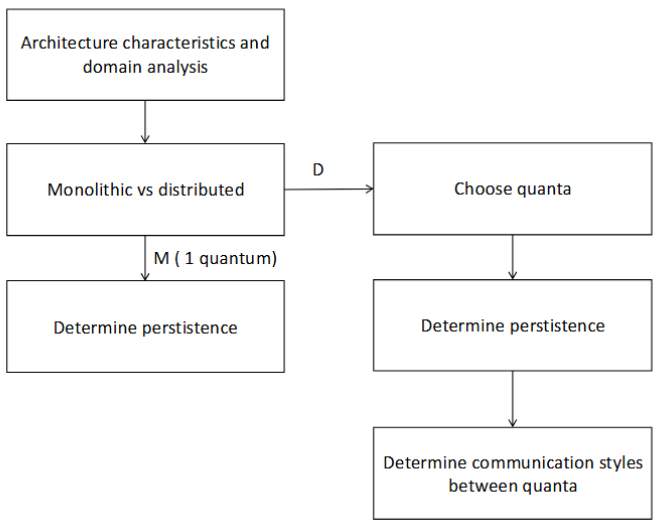
\includegraphics[width=\linewidth]{content/chapters/images/2026-04-25-11-40-35.png}
    \captionof{figure}{Scoping}
  \end{minipage}
\end{flushleft}


\section{Architectural styles}

\begin{itemize}
  \item Monolithic = single deployment unit of all code
  \item One architectural quantum
  \item Distributed = multiple deployment units connected through remote access protocols
\end{itemize}


\begin{table}[h!]
  \renewcommand{\arraystretch}{1.4}
  \centering
  \begin{tabular}{l l }
    \toprule
    \textbf{Monolithic}       & \textbf{Distributed} \\
    \midrule
    Layered architecture      & Service-based        \\
    Pipeline architecture     & Event-driven         \\
    Modular monolithic style  & Space-based          \\
    Micro-kernel architecture & Service-oriented     \\
                              & Microservices        \\
    \bottomrule
  \end{tabular}
\end{table}



\section{Layered architecture - n tier}

Also known as n-tier architecture. Technical partioning.
Each layer is independent and has a specific responsibility.
A layer represents a function of the system.
Pro: testability

Common patterns are:
\begin{itemize}
  \item Presentation layer
  \item Business logic layer
  \item Persistence layer
  \item Database layer
\end{itemize}


In the layered architecture, the layers can communicate only with the adjacent layers.
Teams needing structured development.

\subsection{Layered architecture - variations}


\begin{figure}[h!]
  \centering
  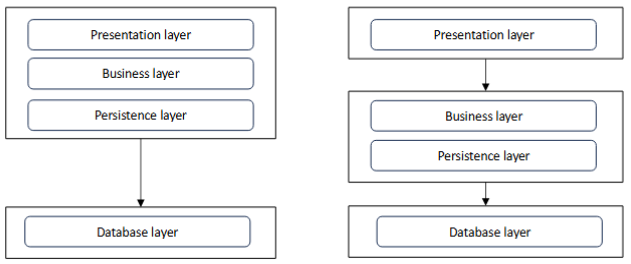
\includegraphics[width=0.25\linewidth]{content/chapters/images/2026-04-25-11-49-01.png}
\end{figure}

\subsection{Addding layers}
New layers to enforce architectural constraints, helps controll access and dependencies.
Example: add \textit{service layer} for share common logic

\subsection{Isolation}
Each layer is indepedent, interacting only through defined contracts.
Prevents tight coupling and cross-layer dependencies.
The risk is the \textbf{Sinkhole antipattern}.

\subsection{Open layers}
Allow direct access to any layer for efficiency, useful for simple
operations. Improves performance but reduces architectural control.


\subsection{Open vs close layers}

\begin{itemize}
  \item Closed layers $\to$ stability, modularity, easier changes
  \item Open layers $\to$ flexibility, performance, but higher risk of coupling
\end{itemize}

Synkholes acceptable threshold: $20\%$  manageable, $80\%$ change architecture style!


\begin{table}[h!]
  \renewcommand{\arraystretch}{1.4}
  \centering
  \begin{tabular}{l l l l}
    \toprule
                & \textbf{Characteristic} & \textbf{Rating} & \textbf{Notes}                  \\
    \midrule
    Structural  & Simplicity              & Very High       &                                 \\
                & Modularity              & Very low        &                                 \\
    \midrule
    Engineering & Maintainability         & Very low        & Changes can impact every layer  \\
                & Testability             & Low             & Mock/stub components            \\
                & Deployability           & Very low        & At every change !               \\
                & Evolvability            & Very low        & Changes can impact every layer  \\
    \midrule
    Operational & Responsiveness          & Medium          & Caching and multithreading      \\
                & Scalability             & Very low        & Lack of modularity              \\
                & Elasticity              & Very low        & Lack of modularity              \\
                & Fault tolerance         & Very low        & Faults impact the whole system, \\
                &                         &                 & all layers must be restarted    \\
    \bottomrule
  \end{tabular}
\end{table}

\begin{table}[h!]
  \renewcommand{\arraystretch}{1.4}
  \centering
  \begin{tabularx}{0.9\textwidth}{X X}
    \toprule
    \textbf{When to use}                                            & \textbf{When not to use}                                 \\
    \midrule
    Applications with clear separation                              & Not ideal for high-performance or highly dynamic systems \\
    Small, simple applications                                      & Large and complex applications                           \\
    As starting point for situations with low budget and short time &                                                          \\
    To quickly test new ideas                                       &                                                          \\
    Examples of usage: operating systems, desktop applications      &                                                          \\
    \bottomrule
  \end{tabularx}
\end{table}


\section{Modular monolithic style}



\begin{center}
  \begin{minipage}{0.65\linewidth}
    Domain partitioned: each module encapsulates a business capability.
    Strong internal boundaries required. Modules with clear responsibilities.
    Deployed as a single unit of software. E.g. Web archive (WAR) file.7

    Modules might have their own dedicated repositories.

    In this we decupled all the modules like Customer, Order, etc.
    The team is also oragnized in different way before a team for each layer,
    now we have a team for each modules or a pool of modules.

    \subsubsection{Data topology}

    Also in this style we can have single database ormore domain-specific databases for the best performance.

    \subsubsection{Interaction between modules}

    The modules \textbf{communicate directly} (peer to peer) or \textbf{through a mediator}
    the gool is orchestrate different modules.

  \end{minipage}%
  \hfill
  \begin{minipage}{0.3\linewidth}
    \centering
    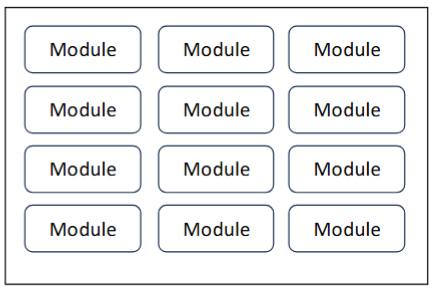
\includegraphics[width=\linewidth]{content/chapters/images/2026-04-25-12-02-42.png}
  \end{minipage}
\end{center}

\subsection{Layered vs modular: components organization}

\begin{itemize}
  \item Layered: com.app.presentation.customer.profile
  \item Modular: com.app.customer.profile; com.app.customer.profile.presentation; \dots
\end{itemize}


\subsection{Variations of modular monolithic style}

\begin{figure}[h!]
  \centering
  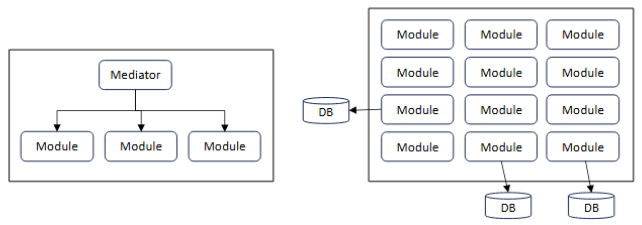
\includegraphics[width=0.3\linewidth]{content/chapters/images/2026-04-25-12-06-52.png}
\end{figure}

\subsection{Advantages and disadvantages of modular monolithic style}

\begin{table}[h!]
  \renewcommand{\arraystretch}{1.4}
  \centering
  \begin{tabularx}{0.9\textwidth}{X X}
    \toprule
    \textbf{Key characteristics}                               & \textbf{Tradeoffs:
                                                                 }                          \\
    \midrule
    Simpler operational model than
    microservices                                              & Risk of becoming tightly coupled over time \\
    No network overhead                                        & Limited independent scalability            \\
    Easier testing and debugging with respect to layered style & Large codebase can slow development        \\
    Requires discipline to maintain boundaries                 & Harder team autonomy at scale              \\
                                                               & Risk of long start up                      \\
    \bottomrule
  \end{tabularx}
\end{table}

\begin{table}[h!]
  \renewcommand{\arraystretch}{1.4}
  \centering
  \begin{tabularx}{0.9\textwidth}{l X X X}
    \toprule
                & \textbf{Characteristic} & \textbf{Modular Monolith} & \textbf{Notes}                                   \\
    \midrule
    Structural  & Simplicity              & Very High                 &                                                  \\
                & Modularity              & Low                       &                                                  \\
    \midrule
    Engineering & Maintainability         & Low                       & Better than Layered because of higher modularity \\
                & Testability             & Low                       & As above                                         \\
                & Deployability           & Low                       & As above                                         \\
                & Evolvability            & Low                       & As above                                         \\
    \midrule
    Operational & Responsiveness          & Medium                    &                                                  \\
                & Scalability             & Very low                  &                                                  \\
                & Elasticity              & Very low                  &                                                  \\
                & Fault tolerance         & Very low                  &                                                  \\
    \bottomrule
  \end{tabularx}
\end{table}


\begin{table}[h!]
  \renewcommand{\arraystretch}{1.4}
  \centering
  \begin{tabularx}{0.9\textwidth}{X X}
    \toprule
    \textbf{When to use}                              & \textbf{When not to use}                                  \\
    \midrule
    Early-stage systems needing structure             & Systems with high demands for operational characteristics \\
    Situations with tight time and budget constraints & Systems requiring independent scaling                     \\
    Teams wanting simplicity over distribution        & When majority of changes are technically-oriented         \\
    Teams working with DDD                            &                                                           \\
    Applications with strong domain boundaries        &                                                           \\
    \bottomrule
  \end{tabularx}
\end{table}

\section{Pipeline architecture}


\begin{center}
  \begin{minipage}{0.65\linewidth}
    Also known as Pipes and Filters.
    Technically partitioned.
    Data flows through a sequence of processing steps.
    Each step transforms input into output.
    Filters are independent and stateless (ideally)

  \end{minipage}%
  \hfill
  \begin{minipage}{0.3\linewidth}
    \centering
    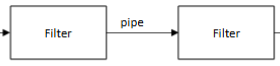
\includegraphics[width=\linewidth]{content/chapters/images/2026-04-25-12-43-02.png}
  \end{minipage}
\end{center}




\begin{flushleft}
  \begin{minipage}{0.65\linewidth}
    \raggedright
    \subsection{Components}

    \begin{itemize}
      \item \textbf{Filters}: processing units performing specific business functions
      \item \textbf{Pipes}: connectors passing data between filters, unidirectionally. Can
            be deployed as remote service (style remains monolith). Can be either
            synchronous or asynchronous (e.g., threads, messages).
      \item \textbf{Data format}: must be consistent or transformed
      \item \textbf{Database}: usually a single db, but filter can have their own database too
      \item \textbf{Producer}: starting point of a process
      \item \textbf{Transformer}: enhance, transform, compute (map)
      \item \textbf{Tester}: test input w.r.t. to criteria (reduce), optionally produces
            output
      \item \textbf{Consumer}: termination point, with persistence
    \end{itemize}
  \end{minipage}%
  \hfill
  \begin{minipage}{0.3\linewidth}
    \centering
    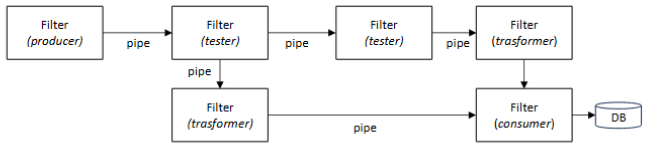
\includegraphics[width=\linewidth]{content/chapters/images/2026-04-25-12-44-57.png}
  \end{minipage}
\end{flushleft}


\begin{table}[h!]
  \renewcommand{\arraystretch}{1.4}
  \centering
  \begin{tabularx}{0.9\textwidth}{X X}
    \toprule
    \textbf{Key characteristics:}    & \textbf{Tradeoffs:}                  \\
    \midrule
    Easy to extend by adding filters & Latency due to multiple stages       \\
    Clear separation of concerns     & Harder debugging across pipeline     \\
    Examples: Bash, Zsh, MapReduce   & Weak fit for complex business logic  \\
                                     & Data format coupling between filters \\
    \bottomrule
  \end{tabularx}
\end{table}

\begin{table}[h!]
  \renewcommand{\arraystretch}{1.4}
  \centering
  \begin{tabularx}{0.9\textwidth}{l X X X}
    \toprule
                & \textbf{Characteristic} & \textbf{Pipeline} & \textbf{Notes}                                                                  \\
    \midrule
    Structural  & Simplicity              & High              &                                                                                 \\
                & Modularity              & Low               & Separation of concerns in filters                                               \\
    \midrule
    Engineering & Maintainability         & Low               &                                                                                 \\
                & Testability             & Medium            & Separation of concerns in filters                                               \\
                & Deployability           & Low               &                                                                                 \\
                & Evolvability            & Medium            &                                                                                 \\
    \midrule
    Operational & Responsiveness          & Medium            &                                                                                 \\
                & Scalability             & Very low          & Separate deployments can improve it, but at the expense of simplicity and cost. \\
                & Elasticity              & Very low          & As above                                                                        \\
                & Fault tolerance         & Very low          & As above                                                                        \\
    \bottomrule
  \end{tabularx}
\end{table}

\begin{table}[h!]
  \renewcommand{\arraystretch}{1.4}
  \centering
  \begin{tabularx}{0.9\textwidth}{X X}
    \toprule
    \textbf{When to use}                                            & \textbf{When not to use}                                        \\
    \midrule
    Data processing and transformation pipelines                    & In systems with non-deterministic flows (use event-driven a.s.) \\
    Streaming or ETL systems                                        & When fault tolerance is important                               \\
    If properly implemented: independent, reusable processing steps & When bi-directional communication is needed                     \\
                                                                    & If high demands of operational characteristics                  \\
    \bottomrule
  \end{tabularx}
\end{table}


\section{Micro-kernel - plug-in architecture style}




\begin{center}
  \begin{minipage}{0.65\linewidth}
    Also known as Plug-in architecture.
    Core system with basic and stable functionalities («happy paths»).
    It can be technically or domain partioned.
    Plug-ins extend system capabilities and incorporate complexity.
    Registry or discovery mechanism.
    Data topology: one db or plug-in specific data sources
  \end{minipage}%
  \hfill
  \begin{minipage}{0.3\linewidth}
    \centering
    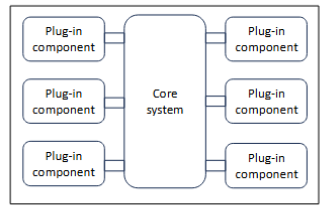
\includegraphics[width=0.7\linewidth]{content/chapters/images/2026-04-25-12-51-42.png}
  \end{minipage}
\end{center}

\subsection{UI: variants}

\begin{figure}[h!]
  \centering
  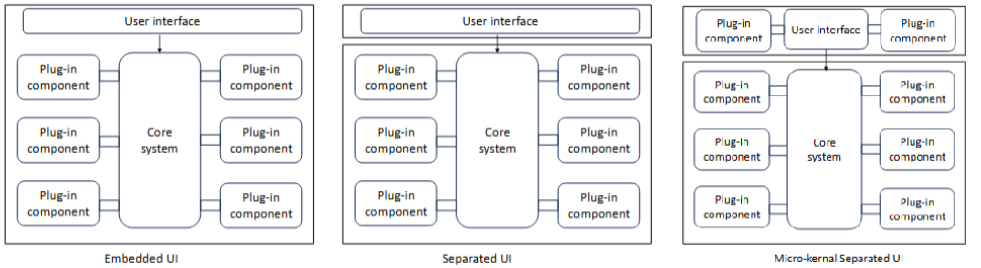
\includegraphics[width=0.5\linewidth]{content/chapters/images/2026-04-25-12-55-06.png}
\end{figure}

\subsection{Plug-in components}
\begin{itemize}
  \item They should be independent and self-contained
  \item Communication p2p with the core system, not between plugins
  \item Compile based vs runtime base
  \item Common semantic, e.g. app.plugin.<domain>.<context> -> Example. app.plugin.editors.plain
  \item Plug-in could a standalone remote service
        \begin{itemize}
          \item The architecture remains monolithic due to coupling with core system
          \item Advantages: scalability, throughput, asynchronous communication
          \item Disdvantages: reliability, costs, complexity
        \end{itemize}
\end{itemize}

\begin{table}[h!]
  \renewcommand{\arraystretch}{1.4}
  \centering
  \begin{tabularx}{0.9\textwidth}{X X}
    \toprule
    \textbf{Characteristics:}            & \textbf{Trade-offs:}                        \\
    \midrule
    Highly extensible and customizable   & Performance overhead from indirection       \\
    Separation between core and features & Complex plug-in lifecycle management        \\
    Supports product variability         & Testing combinations of plugins can be hard \\
    Stable core is critical              & Core design mistakes are costly             \\
    \bottomrule
  \end{tabularx}
\end{table}


\begin{table}[h!]
  \renewcommand{\arraystretch}{1.4}
  \centering
  \begin{tabularx}{0.9\textwidth}{X X}
    \toprule
    \textbf{When to use}                & \textbf{When not to use}                \\
    \midrule
    Common Product-based systems        & Core systems that need frequent changes \\
    Systems requiring extensibility     & High dependencies between plugins       \\
    Platforms with plugin ecosystems    &                                         \\
    Customization-driven applications   &                                         \\
    Examples: browsers, IDEs, PMD, Jira &                                         \\
    \bottomrule
  \end{tabularx}
\end{table}

\begin{table}[h!]
  \renewcommand{\arraystretch}{1.4}
  \centering
  \begin{tabularx}{0.9\textwidth}{l X X X}
    \toprule
                & \textbf{Characteristic} & \textbf{Microkernel} & \textbf{Notes}                                                    \\
    \midrule
    Structural  & Simplicity              & High                 &                                                                   \\
                & Modularity              & Medium               & Extensions easier with plugins                                    \\
    \midrule
    Engineering & Maintainability         & Medium               & Functionalities are better isolated w.r.t other monolithic styles \\
                & Testability             & Medium               & As above                                                          \\
                & Deployability           & Medium               & As above                                                          \\
                & Evolvability            & Medium               & Extensions easier with plugins                                    \\
    \midrule
    Operational & Responsiveness          & Medium               & Microkernel applications are generally small                      \\
                & Scalability             & Very low             &                                                                   \\
                & Elasticity              & Very low             &                                                                   \\
                & Fault tolerance         & Very low             &                                                                   \\
    \bottomrule
  \end{tabularx}
\end{table}

\section{Monolithic Styles - recap}

\begin{table}[h!]
  \renewcommand{\arraystretch}{1.4}
  \centering
  \begin{tabularx}{\textwidth}{l l l l l l}
    \toprule
                & \textbf{Characteristic} & \textbf{Layered (n-tier)} & \textbf{Modular Monolith} & \textbf{Pipeline} & \textbf{Microkernel} \\
    \midrule
    Structural  & Simplicity              & Very High                 & Very High                 & High              & High                 \\
                & Modularity              & Very low                  & Low                       & Low               & Medium               \\
    \midrule
    Engineering & Maintainability         & Very low                  & Low                       & Low               & Medium               \\
                & Testability             & Low                       & Low                       & Medium            & Medium               \\
                & Deployability           & Very low                  & Low                       & Low               & Medium               \\
                & Evolvability            & Very low                  & Low                       & Medium            & Medium               \\
    \midrule
    Operational & Responsiveness          & Medium                    & Medium                    & Medium            & Medium               \\
                & Scalability             & Very low                  & Very low                  & Very low          & Very low             \\
                & Elasticity              & Very low                  & Very low                  & Very low          & Very low             \\
                & Fault tolerance         & Very low                  & Very low                  & Very low          & Very low             \\
    \bottomrule
  \end{tabularx}
\end{table}
